% Editable source for prior_ratios.pdf (pdflatex prior_ratios.tex).
% Prior rho/IC online ratios that this Tier 1 protocol re-measures. Values from the cited records.
\documentclass[border=6pt]{standalone}
\usepackage[T1]{fontenc}
\usepackage{pgfplots}
\pgfplotsset{compat=1.18}
\begin{document}
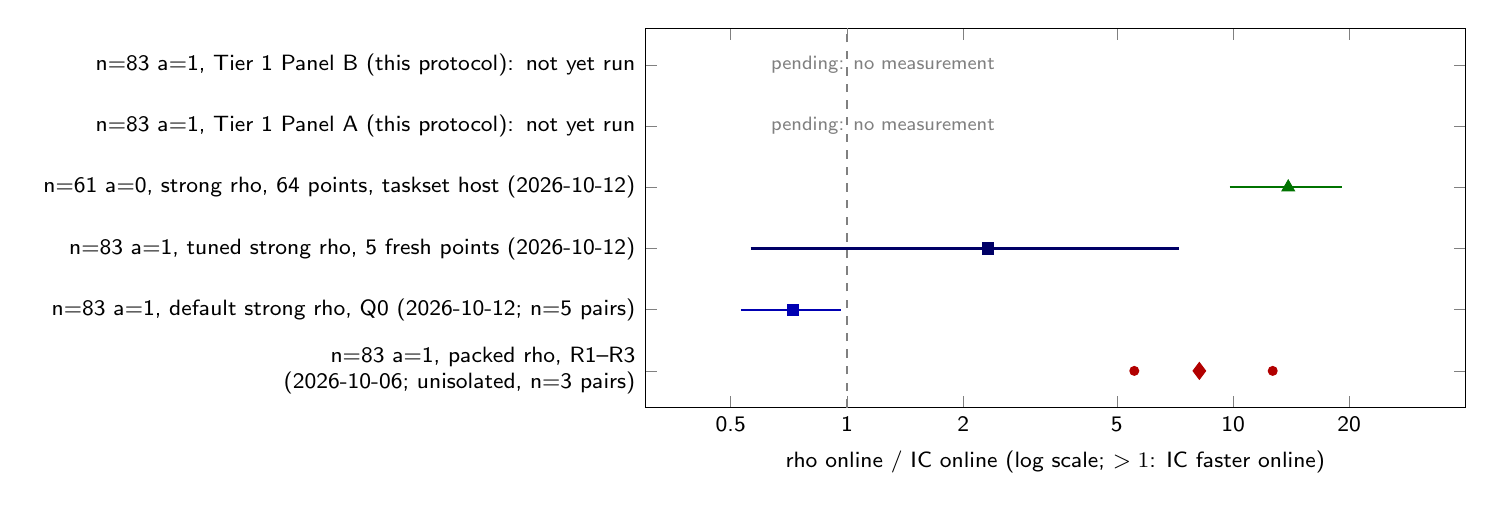
\begin{tikzpicture}
\begin{axis}[
  xmode=log, width=12cm, height=6.4cm, font=\sffamily\footnotesize,
  xmin=0.3, xmax=40, ymin=0.4, ymax=6.6,
  xlabel={rho online / IC online (log scale; $>1$: IC faster online)},
  ytick={1,2,3,4,5,6},
  yticklabels={
    {n=83 a=1, packed rho, R1--R3 (2026-10-06; unisolated, n=3 pairs)},
    {n=83 a=1, default strong rho, Q0 (2026-10-12; n=5 pairs)},
    {n=83 a=1, tuned strong rho, 5 fresh points (2026-10-12)},
    {n=61 a=0, strong rho, 64 points, taskset host (2026-10-12)},
    {n=83 a=1, Tier 1 Panel A (this protocol): not yet run},
    {n=83 a=1, Tier 1 Panel B (this protocol): not yet run}},
  yticklabel style={align=right,text width=7.6cm},
  xtick={0.5,1,2,5,10,20}, xticklabels={0.5,1,2,5,10,20},
  extra x ticks={1}, extra x tick labels={}, extra x tick style={grid=major,grid style={dashed,gray}},
  ]
% packed rho: individual ratios (dots) and median (diamond)
\addplot[only marks,mark=*,mark size=1.6pt,red!70!black] coordinates {(8.181,1) (5.550,1) (12.671,1)};
\addplot[only marks,mark=diamond*,mark size=3pt,red!70!black] coordinates {(8.181,1)};
% default strong: geometric mean strong/IC = 1/1.382330 with interval 1/[1.882300,1.035774]
\addplot[only marks,mark=square*,mark size=2pt,blue!70!black] coordinates {(0.723416,2)};
\draw[blue!70!black,thick] (axis cs:0.531265,2) -- (axis cs:0.965461,2);
% tuned strong: IC/selected geometric ratio 0.431011 [0.137988,1.776388] -> rho/IC 2.320 [0.563,7.247]
\addplot[only marks,mark=square*,mark size=2pt,blue!40!black] coordinates {(2.320127,3)};
\draw[blue!40!black,thick] (axis cs:0.562943,3) -- (axis cs:7.246999,3);
% n=61 isolated: median 13.9 [9.8,19.1]
\addplot[only marks,mark=triangle*,mark size=2.6pt,green!45!black] coordinates {(13.9,4)};
\draw[green!45!black,thick] (axis cs:9.8,4) -- (axis cs:19.1,4);
\node[gray,anchor=west,font=\sffamily\scriptsize] at (axis cs:0.6,5) {pending: no measurement};
\node[gray,anchor=west,font=\sffamily\scriptsize] at (axis cs:0.6,6) {pending: no measurement};
\end{axis}
\end{tikzpicture}
\end{document}
